\documentclass[12pt,letterpaper]{article}
\usepackage{preamble}

%%%%%%%%%%%%%%%%%%%%%%%%%%%%%%%%%%%%%%%%%%
%%%% Edit These for yourself
%%%%%%%%%%%%%%%%%%%%%%%%%%%%%%%%%%%%%%%%%%
\newcommand\course{}
\newcommand\hwnumber{1}
\newcommand\userID{Pedro R. F de Carvalho}

\documentclass[tikz]{standalone}
\usepackage{pgfgantt}
%\usepackage{tikz}
\usetikzlibrary{shapes.geometric, arrows}
\tikzstyle{tp1} = [rectangle, rounded corners, minimum width=3cm, minimum height=1cm,text centered, draw=black, fill=orange!30]
\tikzstyle{tp2y} = [rectangle, minimum width=3cm, minimum height=1cm, text centered, draw=black, fill=green!30]
\tikzstyle{tp2n} = [rectangle, minimum width=3cm, minimum height=1cm, text centered, draw=black, fill=red!30]
\tikzstyle{tp3} = [rectangle, minimum width=3cm, minimum height=1cm, text centered, draw=black, fill=blue!30]

\tikzstyle{arrow} = [thick,->,>=stealth]

\begin{document}
\textbf{\Large Project: Spinodal and binodal lines for Lennard-Jones and Dignon potentials }

\tableofcontents

\section{The Quesiton}
This projects main goal is to determine the binodal and spinodal lines in the ($\rho \times T$) phase space for systems composed by beads or chains, where those elements will interact through Lennard-Jones or Dignon potential. 

\section{The Systems}
The planned simulations are intendend to emulate the properties of proteic systems, where the protein representation is made in a coarse-graines approach. Here we consider each residue as a bead, those beads can be thethered by harmonic potential \ref{chains} or in a monomeric composition \ref{beads}. Non-chained beads can interact by a simple Lennard-Jones system \ref{LJ Potential}, or by a more realistic sequence-depent approach using the Dignon Potential\ref{DG Potential} where there will also be included electrical charges, and thus electrical potential, as well.
\subsection{Lennard-Jones Potential}\label{LJ Potential}
The Lennard-Jones potential is a canonical potential, defined by the following expression:
\begin{equation}
V(r) = 4 \epsilon \bigg[ \bigg(\frac{\sigma}{r}\bigg)^{12}  - \bigg(\frac{\sigma}{r}\bigg)^{6} \bigg]
\end{equation}

Where,

\begin{itemize}
\item $V =$ intermolecular potential.
\item $\sigma =$ distance where V is 0.
\item $r$ = distance between atoms, measured from one center to the other.
\item $\epsilon$ = interaction strength.
\end{itemize}
In computational simulations, in order to save computational time, it is also necessary to define a \textit{cutoff radius} ($r_c$), for which $r\geq r_c \to V(r)=0$.


Here the units will be given as function of the Lennard-Jones parameters:
\begin{itemize}
\item mass = $m$
\item distance = $\sigma$, where $x* = \frac{x}{\sigma}$
\item temperature = $T^* = \frac{T k_b}{\epsilon}$
\item density = $\rho^* = \rho \sigma^3 $
\end{itemize}
   
\subsection{Dignon Scheme}\label{DG scheme}
The Dignon Potential uses a more realistic approach, in his model they apply a sequence-dependent coarse-grain method, where they consider each type of amnioacid as having distinct mass, size, electrical charge and hydrophobic parameter.
\subsubsection{Electrostatic Interaction}\label{electric}
The electrostatic interaction is defined by a Coulombic interaction potential:

\begin{equation}
E_{ij}\left(r\right) = \frac{q_i q_j}{4\pi D r}\exp(-r/\kappa)
\end{equation}

Where:
\begin{itemize}
\item $q_i$ = charge of the ith-aminoacid 
\item $D$ = 80 , Dielectric constant
\item $\kappa$ = 1 nm, Debye screening length
\end{itemize}
\subsubsection{Interaction Potential}\label{dg potential}
Another way the beads interact with themselves is by interaction potential, in this model, this is made by the \textbf{Hidrophobicity scale model}, given by
\begin{equation}
\Phi(r) = 
     \begin{cases}
       &\Phi_{LJ}+(1-\lambda)\epsilon   ,   \text{    if }r\leq 2^{1/6}\sigma}\\
       &\lambda\Phi_{LJ} ,    \text{otherwise}\\
     \end{cases}
\end{equation}
\subsubsection{Parameters Tables}
As previously stated, the Dignon model carries a sequence dependent behavior, which means that for every different type of residues, different parameters are addressed, those sequence-dependent parameters are: mass,$q$,$\lambda$ and $\sigma$ and are given in the following table:
\begin{figure}[!htbp]
\includegraphics[scale=0.7]{images/dgtable.png} 
\caption{Dignon Parameters Table.}
\end{figure}

\subsection{Beads}\label{beads}
Here, everytime we refer to a \textit{bead system}, we are talking about monomeric systems, composed of single beads, interacting using the \textit{Dignon Scheme}\ref{DG scheme} or the \textit{LJ pontential}\ref{LJ Potential}.
\subsection{Chains}\label{chains}
For chained systems,we use the harmonic potential, which in LAMMPS is written as:

\begin{equation}
E=K(r-r_0)^2
\end{equation}

 where:

\begin{itemize}
\item $K$: spring constant
\item $r_0$: relaxed position
\end{itemize}

\textbf{LJ system:}

\begin{itemize}
\item $K=37,500 \epsilon/\sigma^2$
\item $r_0=\sigma$
\end{itemize}

Here we will follow the reference [REF Silmore 2016]. 

\textbf{Dignon system:}

\begin{itemize}
\item $K=10 kJ/\angstrom^2$
\item $r_0=3.8 \angstrom$
\end{itemize}

Here we will follow the reference [REF Dignon Seq-dependent]. 

\section{The Binodal}\label{binodal}
The binodal line is also known as the \textit{coexistence curve}, and indicate the limits of metastability of the system, and it is given by the condition:
\begin{equation}\label{binodalcondition}
\mu_{1}\left(\rho,T\right)=\mu_{2}\left(\rho,T\right)
\end{equation}
inside the metastability region the system is driven through a slow process of aggregation, called nucleation, where the system phase separate in regions of densities $\rho_1$ and $\rho_2$ in order to obey the eq.\ref{binodalcondition}. It is important to stress the fact that, this phenomenom happens in a different timescale than the stabilization of a homogeneous system.
\subsection{The Slab Method}\label{slab method}
The slab method proposes a way to speed-up the phase separation process, allowing the sytem to reach the coexistence densities faster.
This method consist of starting with a large box, compressing it to a dense system and a expansion of the box in a single direction, creating a favourable condition for a phase separated configuration. Summarizing, they leave a dense cluster on a slab with overall density inside the metastable region, the cluster will dissolve until it reaches the coexistence densities, given by the densities inside and outside the cluster.
\begin{figure}[!htbp]
\includegraphics[height=\textwidth, angle =90 ]{images/Screeshot_beads_slab.png} 
\caption{Snapshot of a system of beads interacting via LJ-potential.}
\end{figure}
\begin{figure}[!htbp]
\includegraphics[width=0.75\textwidth]{images/PD.png} 
\caption{Coexistence curve obtained through slab method.}
\end{figure}
\section{The Spinodal}\label{spinodal}
The spinodal curve delimeters the region of instability of the system and is marked by the divergence
or peaks of some response functions, inside the spinodal region the systems is governed by a global
instability, this global instability gives rise to a phase separation known as spinodal decomposition . In
the spinodal decompostion the system will actively phase separate because miscibility is energetically
more expensive than the heterogeneous state, this instability will result in negative values of some
response functions of the system.


\textbf{\textcolor{red}{Following two sections are blank, please refer to the Cv report.}}
\subsection{The Specific Heat Criterion}\label{specific heat}
\begin{figure}[!htbp]
\includegraphics[width=0.75\textwidth]{images/PDTE2.png} 
\caption{spinodal curve obtained through $C_v$ criterion.}
\end{figure}
\subsection{The Cluster Radius Criterion}\label{cluster radius}
\section{Organogram}
In this section we summaraize the systems to be simulated and the current availability of codes.

Where:

\begin{itemize}
\item [\textbf{Random}:] Randomnly disrtibuted residues
\item [\textbf{No q}:] Randomnly disrtibuted residues, excluding charged ones
\item [\textbf{Single}:] One type of residue only
\end{itemize}

It is important to stress that each of thoses boxes represent one type of simulation, which would need to be simulated for different values of temperature for the \textit{slab} method, and for different values of density and temperature for the \textit{Box} simulations.

\newline

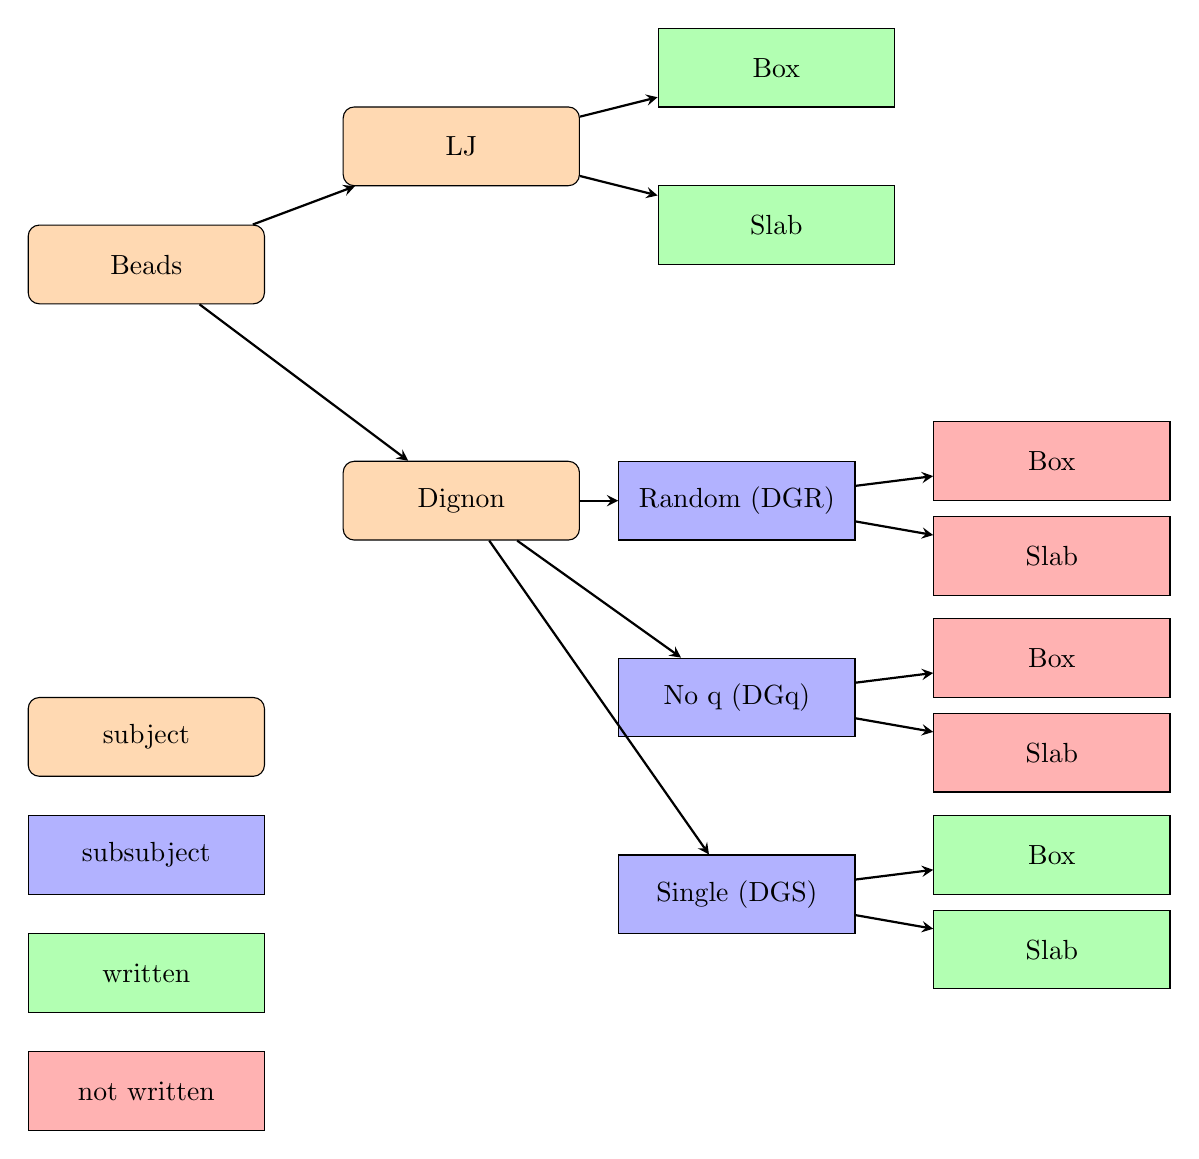
\begin{tikzpicture}[node distance=3cm]

%Boxes
\node (beads) [tp1] {Beads};
%LJ
\node (LJ) [tp1, right of=beads,yshift=1.5cm, xshift=1.0cm] {LJ};
\node (LJbox) [tp2y, right of=LJ, xshift=1.0cm, yshift=1.0cm] {Box};
\node (LJslab) [tp2y, below of=LJbox, yshift=1.0cm] {Slab};
%subtitles
\node (label1) [tp1, below of=beads,yshift=-3cm] {subject};
\node (label2) [tp3, below of=label1,yshift=1.5cm] {subsubject};
\node (label3) [tp2y, below of=label2,yshift=1.5cm] {written};
\node (label4) [tp2n, below of=label3,yshift=1.5cm] {not written};
%Dignon
\node (DG) [tp1, below of=LJ, yshift=-1.5cm] {Dignon};
%Random
\node (DGr) [tp3, right of=DG, xshift=0.5cm] {Random (DGR)};
\node (DGrbox) [tp2n, right of=DGr, xshift=1.0cm, yshift=0.5cm] {Box};
\node (DGrslab) [tp2n, below of=DGrbox, yshift=1.8cm] {Slab};
%No q
\node (DGnq) [tp3, below of=DGr, yshift=0.5cm] {No q (DGq)};
\node (DGnqbox) [tp2n, right of=DGnq, xshift=1.0cm, yshift=0.5cm] {Box};
\node (DGnqslab) [tp2n, below of=DGnqbox, yshift=1.8cm] {Slab};
%Single
\node (DGs) [tp3, below of=DGnq, yshift=0.5cm] {Single (DGS)};
\node (DGsbox) [tp2y, right of=DGs, xshift=1.0cm, yshift=0.5cm] {Box};
\node (DGsslab) [tp2y, below of=DGsbox, yshift=1.8cm] {Slab};

%arrows
\draw [arrow] (beads) -- (LJ);
\draw [arrow] (beads) -- (DG);
\draw [arrow] (LJ) -- (LJbox);
\draw [arrow] (LJ) -- (LJslab);
\draw [arrow] (DG) -- (DGr);
\draw [arrow] (DG) -- (DGnq);
\draw [arrow] (DG) -- (DGs);
\draw [arrow] (DGr) -- (DGrbox);
\draw [arrow] (DGr) -- (DGrslab);
\draw [arrow] (DGnq) -- (DGnqbox);
\draw [arrow] (DGnq) -- (DGnqslab);
\draw [arrow] (DGs) -- (DGsbox);
\draw [arrow] (DGs) -- (DGsslab);


\end{tikzpicture}

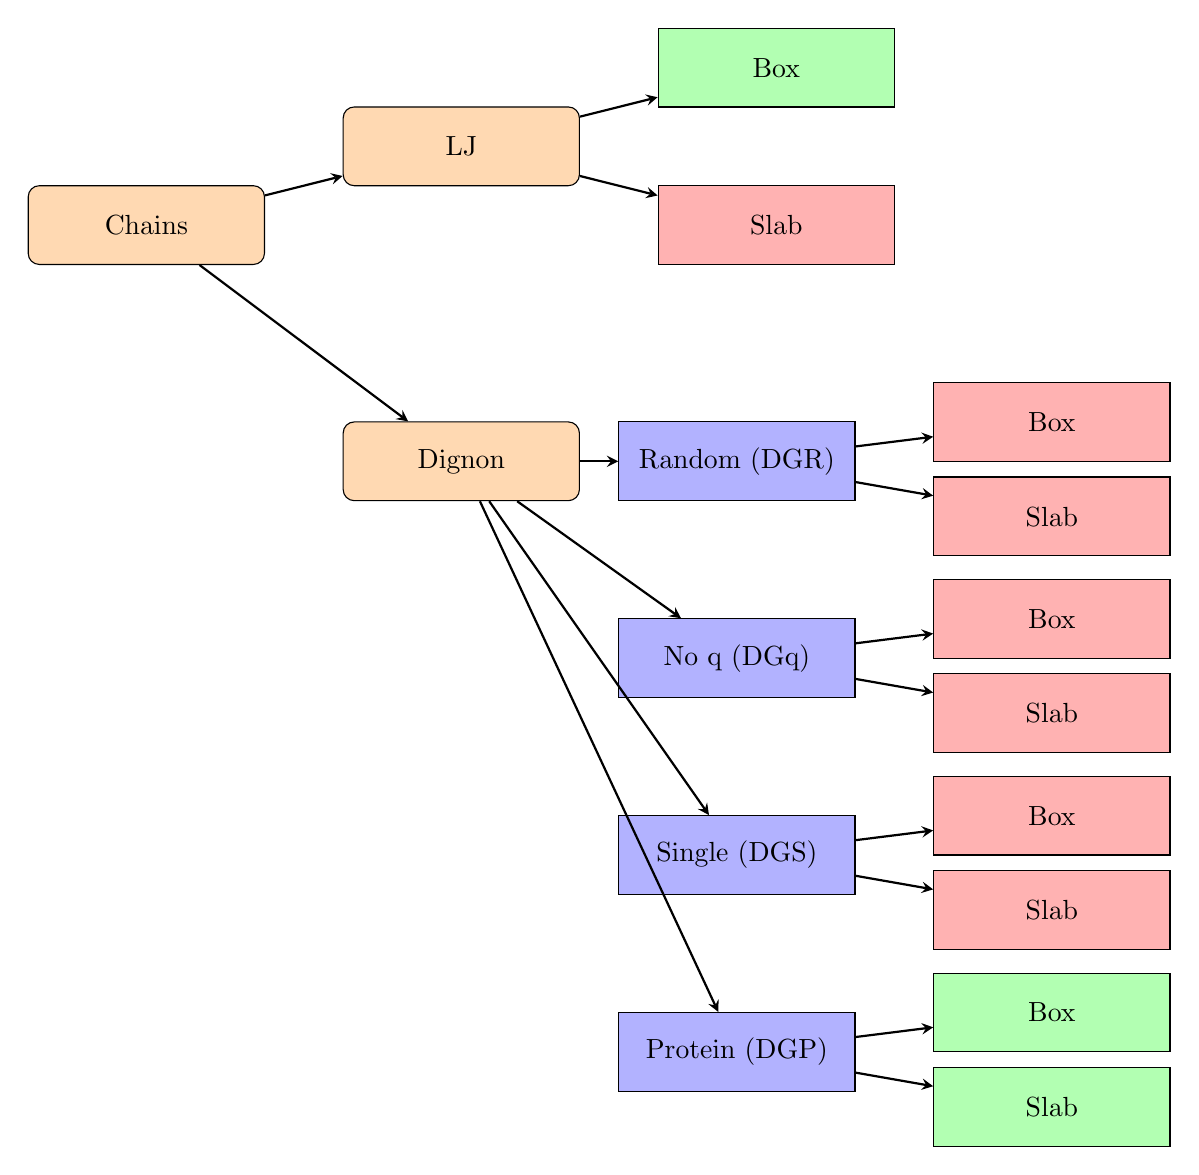
\begin{tikzpicture}[node distance=3cm]

%Boxes
\node (beads) [tp1] {Chains};
%LJ
\node (LJ) [tp1, right of=beads,yshift=1cm, xshift=1.0cm] {LJ};
\node (LJbox) [tp2y, right of=LJ, xshift=1.0cm, yshift=1.0cm] {Box};
\node (LJslab) [tp2n, below of=LJbox, yshift=1.0cm] {Slab};
%Dignon
\node (DG) [tp1, below of=LJ, yshift=-1cm] {Dignon};
%Random
\node (DGr) [tp3, right of=DG, xshift=0.5cm] {Random (DGR)};
\node (DGrbox) [tp2n, right of=DGr, xshift=1.0cm, yshift=0.5cm] {Box};
\node (DGrslab) [tp2n, below of=DGrbox, yshift=1.8cm] {Slab};
%No q
\node (DGnq) [tp3, below of=DGr, yshift=0.5cm] {No q (DGq)};
\node (DGnqbox) [tp2n, right of=DGnq, xshift=1.0cm, yshift=0.5cm] {Box};
\node (DGnqslab) [tp2n, below of=DGnqbox, yshift=1.8cm] {Slab};
%Single
\node (DGs) [tp3, below of=DGnq, yshift=0.5cm] {Single (DGS)};
\node (DGsbox) [tp2n, right of=DGs, xshift=1.0cm, yshift=0.5cm] {Box};
\node (DGsslab) [tp2n, below of=DGsbox, yshift=1.8cm] {Slab};
%Protein
\node (DGp) [tp3, below of=DGs, yshift=0.5cm] {Protein (DGP)};
\node (DGpbox) [tp2y, right of=DGp, xshift=1.0cm, yshift=0.5cm] {Box};
\node (DGpslab) [tp2y, below of=DGpbox, yshift=1.8cm] {Slab};

%arrows
\draw [arrow] (beads) -- (LJ);
\draw [arrow] (beads) -- (DG);
\draw [arrow] (LJ) -- (LJbox);
\draw [arrow] (LJ) -- (LJslab);
\draw [arrow] (DG) -- (DGr);
\draw [arrow] (DG) -- (DGnq);
\draw [arrow] (DG) -- (DGs);
\draw [arrow] (DG) -- (DGp);
\draw [arrow] (DGr) -- (DGrbox);
\draw [arrow] (DGr) -- (DGrslab);
\draw [arrow] (DGnq) -- (DGnqbox);
\draw [arrow] (DGnq) -- (DGnqslab);
\draw [arrow] (DGs) -- (DGsbox);
\draw [arrow] (DGs) -- (DGsslab);
\draw [arrow] (DGp) -- (DGpbox);
\draw [arrow] (DGp) -- (DGpslab);

\end{tikzpicture}

\newpage

\section{Jobs}
\subsection{Beads}
\subsubsection{LJ Box}
\begin{itemize}
\item	1 Temperature
\item	50 densities
\item	2916 beads
\item	Total Wall Time: $20:35$
\end{itemize}
\subsubsection{LJ Slab}
\begin{itemize}
\item	1 Temperature
\item	1 initial density
\item	2916 beads
\item	Total Wall Time: $8:10$
\end{itemize}



\section{Timeline of this project}\label{timeline}



%
% A fairly complicated example from section 2.9 of the package
% documentation. This reproduces an example from Wikipedia:
% http://en.wikipedia.org/wiki/Gantt_chart
%
\title{Gantt Charts with the pgfgantt Package}
\definecolor{barblue}{RGB}{153,204,254}
\definecolor{groupblue}{RGB}{51,102,254}
\definecolor{linkred}{RGB}{165,0,33}
\renewcommand\sfdefault{phv}
\renewcommand\mddefault{mc}
\renewcommand\bfdefault{bc}
%REF LINKS
%\setganttlinklabel{s-s}{START-TO-START}
%\setganttlinklabel{f-s}{FINISH-TO-START}
%\setganttlinklabel{f-f}{FINISH-TO-FINISH}
\sffamily
\begin{ganttchart}[
	x unit=0.8cm,
    canvas/.append style={fill=none, draw=black!5, line width=.75pt},
    hgrid style/.style={draw=black!5, line width=.75pt},
    vgrid={*1{draw=black!5, line width=.75pt}},
    today=1,
    today rule/.style={
      draw=black!64,
      dash pattern=on 3.5pt off 4.5pt,
      line width=1.5pt
    },
    today label font=\small\bfseries,
    title/.style={draw=none, fill=none},
    title label font=\bfseries\footnotesize,
    title label node/.append style={below=7pt},
    include title in canvas=false,
    bar label font=\mdseries\small\color{black!70},
    bar label node/.append style={left=2cm},
    bar/.append style={draw=none, fill=red!63},
    bar incomplete/.append style={fill=barblue},
    bar progress label font=\mdseries\footnotesize\color{black!70},
    group incomplete/.append style={fill=groupblue},
    group left shift=0,
    group right shift=0,
    group height=.5,
    group peaks tip position=0,
    group label node/.append style={left=.6cm},
    group progress label font=\bfseries\small,
    link/.style={-latex, line width=1.5pt, linkred},
    link label font=\scriptsize\bfseries,
    link label node/.append style={below left=-2pt and 0pt}
  ]{1}{16}
  
  \gantttitle[title label node/.append style={below left=7pt and -3pt}
  ]{WEEKS:\quad1}{1}
  \gantttitlelist{2,...,16}{1} \\
  \ganttgroup[progress=10]{Beads}{1}{12} \\
  \ganttbar[progress=75,progress label text={},name=LJBox]{\textbf{LJ} Box}{1}{2} \\  
  \ganttbar[progress=75,progress label text={},name=LJSlab]{\textbf{LJ} Slab}{1}{2} \\
  \ganttbar[progress=75,progress label text={}]{\textbf{DGR} Box}{8}{10} \\
  \ganttbar[progress=75,progress label text={}]{\textbf{DGR} Slab}{8}{9} \\
  \ganttbar[progress=75,progress label text={}]{\textbf{DGq} Box}{12}{14} \\
  \ganttbar[progress=75,progress label text={}]{\textbf{DGq} Slab}{12}{13} \\
  \ganttbar[progress=75, progress label text={}]{\textbf{DGS} Box}{6}{8}\\
  \ganttbar[progress=75,progress label text={}]{\textbf{DGS} Slab}{6}{7} \\[grid]
  \ganttgroup[progress=0]{Chains}{2}{16} \\
  \ganttbar[progress=75,progress label text={}]{\textbf{LJ} Box}{2}{5} \\
  \ganttbar[progress=75,progress label text={}]{\textbf{LJ} Slab}{3}{6} \\
  \ganttbar[progress=75,progress label text={}]{\textbf{DGR} Box}{10}{12} \\
  \ganttbar[progress=75,progress label text={}]{\textbf{DGR} Slab}{10}{11} \\
  \ganttbar[progress=75,progress label text={}]{\textbf{DGq} Box}{14}{16} \\
  \ganttbar[progress=75,progress label text={}]{\textbf{DGq} Slab}{14}{16} \\
  \ganttbar[progress=75,progress label text={}]{\textbf{DGP} Box}{14}{16} \\
  \ganttbar[progress=75,progress label text={}]{\textbf{DGP} Slab}{14}{16} \\
  \ganttbar[progress=75,progress label text={}]{\textbf{DGS} Box}{4}{7} \\
  \ganttbar[progress=75,progress label text={}]{\textbf{DGS} Slab}{4}{6} 
	%DRAW LINKS  
  %\ganttlink[link type=s-s]{WBS1A}{WBS1B}
  %\ganttlink[link type=f-s]{WBS1B}{WBS1C}
  %\ganttlink[link type=f-f,link label node/.append style=left]{WBS1C}{WBS1D}
\end{ganttchart}


\section{Codelist(Outdated)}
(THIS SECTION BELLOW IS OLD, IT WILL BE FIXED SOON)
Right now I have:
\begin{itemize}
            \item [$Dignon\_slab$]  folder with the Dignon chain slab method.
			\item [$LJ\_chain.lmp$]  box simulation of LJ chains
			\item [$slab\_long.lmp$]  slab simulation for LJ beads
			\item [$in.P-simplelj$]  box simulation for LJ beads
\end{itemize}

To check:

\begin{itemize}
			\item in.dignon_fluid_box : dignon fluid box simulation
\end{itemize}			
		
Missing:

\begin{itemize}
\item slab simulation of LJ chains
\end{itemize}  
  
\bibliographystyle{plain}
\bibliography{bibfile}
\end{document}


%TRASH

%
% A simpler example from the package documentation:
%
%\begin{ganttchart}{1}{12}
%  \gantttitle{2011}{12} \\
%  \gantttitlelist{1,...,12}{1} \\
%  \ganttgroup{Group 1}{1}{7} \\
%  \ganttbar{Task 1}{1}{2} \\
%  \ganttlinkedbar{Task 2}{3}{7} \ganttnewline
%  \ganttmilestone{Milestone}{7} \ganttnewline
%  \ganttbar{Final Task}{8}{12}
%  \ganttlink{elem2}{elem3}
%  \ganttlink{elem3}{elem4}
%\end{ganttchart}
